\mychapter{Resultados} 
\label{Cap:Resultados}

Neste capítulo, são apresentados os resultados da implementação e testes do \textit{software} RADARE, com foco na precisão dos dados reconciliados, no desempenho computacional em diferentes cenários de carga e na usabilidade da ferramenta, tanto no \textit{front-end} (menu e \textit{canvas}) quanto no \textit{back-end} (rotas, serviços e banco de dados). Além disso, foram desenvolvidos dois manuais: um para a manutenção técnica do sistema e outro para orientar o uso pelos usuários finais.

Para facilitar a leitura e não quebrar a dinâmica do texto principal, todos os códigos desenvolvidos para o RADARE foram incluídos nos Apêndices. Devido à sua extensão, a decisão de alocar os trechos de código nos Apêndices permite uma melhor fluidez no corpo do trabalho. Sempre que um código for citado ao longo do texto, será indicada a referência ao apêndice correspondente para consulta detalhada.

% -------------------------
\section{Resultados do desenvolvimento do \textit{front-end}} 

O \textit{front-end} do projeto  foi desenvolvido com foco em oferecer uma interface intuitiva, visando otimizar a interação dos usuários com a ferramenta de modelagem. A interface facilita a visualização dos fluxos de dados e dos modelos, além de permitir a execução da reconciliação. O  \textit{front-end} do sistema é estruturado em duas áreas principais: o menu, responsável pelo gerenciamento das ações e funcionalidades, e o \textit{canvas}, onde os nódulos conectados podem ser visualizados e manipulados diretamente pelos usuários.

% -------------------------
\subsection{Menu de controle da interface gráfica} 

A sessão de menu do RADARE apresenta ao usuário uma interface de fácil interação, permitindo a adição de componentes, o controle do fluxo de dados e o gerenciamento da visualização geral do sistema. Cada funcionalidade disponível no menu é descrita de maneira detalhada nas subseções a seguir, acompanhada por exemplos de código e imagens que ilustram sua implementação no contexto da ferramenta.

A biblioteca \textit{ReactFlow} \cite{reactflow} é fundamental para a manipulação dos nódulos no \textit{canvas} e foi significativamente adaptada para atender às necessidades específicas do projeto. As modificações realizadas garantem uma usabilidade eficiente, permitindo que os usuários adicionem e conectem os nódulos de forma dinâmica, com fluidez e precisão.

Cada nódulo inserido no \textit{canvas} possui uma estrutura personalizada, onde as conexões, denominadas \textit{handles}, são configuradas com características específicas, como estilo visual e lógica de interação. Essa personalização assegura que a visualização dos fluxos de dados seja clara e que sua manipulação seja intuitiva, facilitando o gerenciamento das operações dentro do sistema.

A Figura \ref{Fig:MenuImage} apresenta o menu principal do sistema, destacando as opções para adição de nódulos ao \textit{canvas}. Através desse menu, o usuário pode inserir diferentes tipos de nódulos, como entradas, saídas e pontos de processamento de dados, além de opções como reconciliação de dados e ajustes de visualização. Cada funcionalidade foi projetada para que o usuário possa construir fluxos de dados industriais de maneira modular e interativa, proporcionando maior flexibilidade no gerenciamento e análise de grandes volumes de dados.

\begin{figure}[htbp]
    \centering
    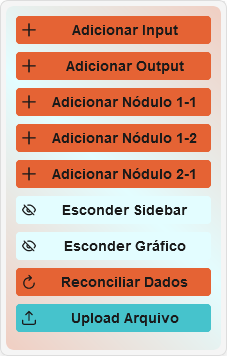
\includegraphics[width=0.4\textwidth]{figuras/menu-image.png}
    \caption{Menu principal do sistema RADARE.}
    \label{Fig:MenuImage}
\end{figure}

\subsubsection{Adicionar Input}

O botão \textbf{"Adicionar Input"} permite ao usuário inserir um novo nódulo de entrada no \textit{canvas}, representando um sensor ou uma fonte de dados no sistema industrial. Ao acionar esse botão, um nó de \textit{input} é adicionado ao \textit{canvas}, possibilitando a conexão desse ponto com outros nódulos do fluxo de dados. A implementação dessa funcionalidade utiliza a biblioteca ReactFlow \cite{reactflow}, o que elimina a necessidade de configurações customizadas iniciais e facilita a criação e manipulação dos nódulos no ambiente visual.

A Figura \ref{Fig:AddInputButton} ilustra o botão "Adicionar Input" na interface gráfica do sistema.

\begin{figure}[htbp]
    \centering
    
\includegraphics[width=0.4\textwidth]{figuras/add-input-button.png}
    \caption{Botão de adicionar input no menu (Fonte: próprio autor, 2024).}
    \label{Fig:AddInputButton}
\end{figure}


\subsubsection{Adicionar output}

O botão \textbf{"Adicionar Output"} permite ao usuário inserir um novo nódulo de saída no \textit{canvas}. Esse \textit{output} representa um destino ou ponto final para os dados no sistema industrial, como a exportação de resultados processados ou a visualização de dados reconciliados. Ao acionar o botão, um novo nó de \textit{output} é adicionado ao \textit{canvas}, possibilitando sua conexão com outros nódulos de processamento ou entrada no fluxo de dados. Assim como ocorre com o \textit{input}, a implementação dessa funcionalidade também utiliza a biblioteca ReactFlow \cite{reactflow}, eliminando a necessidade de customização de comportamentos iniciais.

A Figura \ref{Fig:AddOutputButton} mostra o botão "Adicionar Output" na interface, permitindo ao usuário inserir nódulos de saída no fluxo de dados.

\begin{figure}[htbp]
    \centering
    
\includegraphics[width=0.4\textwidth]{figuras/add-output-button.png}
    \caption{Botão de adicionar output no menu (Fonte: próprio autor, 2024).}
    \label{Fig:AddOutputButton}
\end{figure}

% -------------------------
\subsubsection{Adicionar nódulo 1-1}

O botão \textbf{"Adicionar Nódulo 1-1"} permite ao usuário inserir um novo nódulo de transição no \textit{canvas}. Esse nódulo atua como um ponto intermediário no fluxo de dados, podendo representar sensores, transformações ou outros elementos de processo. Ao clicar no botão, o nódulo é adicionado ao \textit{canvas}, permitindo ao usuário conectá-lo com outros nódulos de forma eficiente.

A lógica para adicionar este nódulo foi desenvolvida de forma personalizada, especificando o tipo de conexão, a quantidade de pontos de conexão (\textit{handles}), além do estilo visual e da posição no \textit{canvas}, garantindo que o comportamento do nódulo se ajuste adequadamente ao fluxo de dados esperado.

O trecho principal do código responsável pela criação desse nódulo, que pode ser encontrado em sua totalidade no \textbf{Anexo \ref{Anexo:frontCodeNodeOneOne}}.
ulo 1-1" disponível no menu do sistema.

\begin{figure}[htbp]
    \centering
    
\includegraphics[width=0.4\textwidth]{figuras/add-node11-button.png}
    \caption{Botão de adicionar Nódulo 1-1 no menu (Fonte: próprio autor, 2024).}
    \label{Fig:AddNodeOneOneButton}
\end{figure}

% -------------------------
\subsubsection{Adicionar nódulo 1-2}

O botão \textbf{"Adicionar Nódulo 1-2"} permite ao usuário inserir um nódulo de transição que recebe uma única entrada e gera duas saídas no \textit{canvas}. Este tipo de nódulo é particularmente útil em cenários onde um único ponto de dados precisa ser bifurcado para diferentes processos ou análises. Ao ser adicionado, o nódulo facilita o roteamento de dados para dois fluxos distintos, mantendo a integridade e a flexibilidade do processo.

A lógica para este nódulo foi customizada para suportar uma conexão de entrada e duas saídas, com o código responsável definindo os \textit{handles} (pontos de conexão), a posição e o estilo visual no \textit{canvas}. Assim como no caso do nódulo 1-1, o comportamento é ajustado para garantir uma integração fluida no fluxo de dados.

O trecho principal do código responsável pela criação desse nódulo pode ser encontrado em sua totalidade no \textbf{Anexo \ref{Anexo:frontCodeNodeOneTwo}}.

A Figura \ref{Fig:AddNodeOneTwoButton} ilustra o botão "Adicionar Nódulo 1-2" disponível no menu do sistema.

\begin{figure}[htbp]
    \centering
    
\includegraphics[width=0.4\textwidth]{figuras/add-node12-button.png}
    \caption{Botão de adicionar Nódulo 1-2 no menu (Fonte: próprio autor, 2024).}
    \label{Fig:AddNodeOneTwoButton}
\end{figure}

\subsubsection{Adicionar nódulo 2-1}

O botão \textbf{"Adicionar Nódulo 2-1"} permite ao usuário inserir um nódulo de transição que recebe duas entradas e gera uma única saída no \textit{canvas}. Esse nódulo é ideal para processos em que múltiplas fontes de dados precisam ser combinadas ou integradas antes de continuar o fluxo. Ao ser adicionado, o nódulo permite a fusão de duas linhas de dados, garantindo que as informações de entrada sejam processadas de forma conjunta antes de seguirem para a próxima etapa.

A lógica para este nódulo foi desenvolvida de maneira personalizada, permitindo a adição de dois pontos de conexão de entrada e um ponto de saída. O código responsável configura os \textit{handles}, define o estilo visual e posiciona o nódulo no \textit{canvas}, assegurando que ele atenda às necessidades de integração e processamento combinados dentro do fluxo de dados.

O trecho principal do código responsável pela criação desse nódulo pode ser encontrado em sua totalidade no \textbf{Anexo \ref{Cap:NodeTwoOneCode}}.

A Figura \ref{Fig:AddNodeTwoOneButton} mostra o botão "Adicionar Nódulo 2-1" presente no menu da interface do sistema.

\begin{figure}[htbp]
    \centering
    
\includegraphics[width=0.4\textwidth]{figuras/add-node21-button.png}
    \caption{Botão de adicionar Nódulo 2-1 no menu (Fonte: próprio autor, 2024).}
    \label{Fig:AddNodeTwoOneButton}
\end{figure}
\subsubsection{Reconciliar dados}

O botão \textbf{"Reconciliar Dados"} executa o processo de reconciliação dos dados conectados no \textit{canvas}. Ao ser acionado, o sistema analisa os nódulos interconectados e realiza a reconciliação dos dados utilizando o método dos multiplicadores de Lagrange. Esse processo ajusta as discrepâncias entre os valores medidos e os valores reconciliados, garantindo que as restrições impostas pelos balanços de massa e energia sejam respeitadas.

A lógica por trás desse botão foi desenvolvida para percorrer os nódulos conectados no \textit{canvas}, extrair os dados necessários e enviá-los ao back-end. No back-end, o algoritmo de reconciliação é executado, processando os dados conforme as regras definidas, e os resultados são retornados ao front-end, onde os dados reconciliados são exibidos no fluxo visual do \textit{canvas}.

O trecho principal do código responsável por essa funcionalidade pode ser encontrado em sua totalidade no \textbf{Anexo \ref{Cap:ReconcileDataCode}}.

A Figura \ref{Fig:ReconcileButton} ilustra o botão "Reconciliar Dados" na interface do sistema.

\begin{figure}[htbp]
    \centering
    
\includegraphics[width=0.4\textwidth]{figuras/reconcile-data-button.png}
    \caption{Botão de reconciliar dados no menu (Fonte: próprio autor, 2024).}
    \label{Fig:ReconcileButton}
\end{figure}

\subsubsection{Esconder gráfico das reconciliações}

O botão \textbf{"Esconder Gráfico das Reconciliações"} permite ao usuário ocultar o gráfico que exibe os resultados das reconciliações de dados, proporcionando uma interface mais organizada e com maior espaço para outros elementos do processo. Ao ativar essa função, o gráfico é temporariamente removido do \textit{dashboard}, mas os dados reconciliados permanecem disponíveis no sistema, permitindo que o usuário possa reexibi-los quando necessário. A lógica implementada para esse botão alterna a visibilidade do gráfico sem interferir nos demais componentes ou no fluxo dos dados processados. O código responsável por essa funcionalidade pode ser encontrado no \textbf{Anexo \ref{Anexo:HideGraphLogic}}.

A Figura \ref{Fig:HideGraphButton} ilustra o botão "Esconder Gráfico das Reconciliações" na interface gráfica.

\begin{figure}[htbp]
    \centering
    
\includegraphics[width=0.4\textwidth]{figuras/hide-graphbar-button.png}
    \caption{Botão de esconder gráfico das reconciliações (Fonte: próprio autor, 2024).}
    \label{Fig:HideGraphButton}
\end{figure}

\subsubsection{Esconder \textit{sidebar} de informações}

O botão \textbf{"Esconder Sidebar de Informações"} permite ao usuário ocultar a barra lateral que exibe informações detalhadas sobre os nódulos e fluxos no \textit{canvas}. Essa barra lateral geralmente contém dados importantes e estatísticas sobre os elementos do processo, sendo especialmente útil para diagnósticos e ajustes detalhados. Ao escondê-la, o usuário ganha mais espaço no \textit{canvas} para manipulação visual, o que é fundamental em fluxos mais complexos, onde a clareza e o espaço visual são prioridades.

A lógica desse recurso foi implementada para alternar a visibilidade da \textit{sidebar} sem que os dados exibidos sejam perdidos. O usuário pode reexibi-la a qualquer momento, com as informações ainda intactas, proporcionando uma interface flexível e adaptável às necessidades específicas de visualização e operação. O código responsável por essa funcionalidade pode ser encontrado no \textbf{Anexo \ref{Anexo:HideSidebarLogic}}.

A Figura \ref{Fig:HideSidebarButton} ilustra o botão "Esconder Sidebar de Informações" na interface gráfica do sistema.

\begin{figure}[htbp]
    \centering
    
\includegraphics[width=0.4\textwidth]{figuras/hide-sidebar-button.png}
    \caption{Botão de esconder a sidebar de informações (Fonte: próprio autor, 2024).}
    \label{Fig:HideSidebarButton}
\end{figure}

\subsubsection{Upload de arquivos em CSV}

O botão \textbf{"Upload de Arquivos CSV"} permite ao usuário importar dados de medições diretamente para o sistema. Esse recurso é fundamental para integrar dados externos ao fluxo de trabalho, possibilitando que arquivos CSV com informações dos sensores e variáveis do processo industrial sejam carregados no RADARE. Após o carregamento, os dados são processados e utilizados nas etapas de reconciliação, facilitando a análise e a correção dos dados.

A funcionalidade foi implementada para garantir o envio e o armazenamento seguro dos arquivos, além de realizar a validação do formato e conteúdo do CSV. Isso assegura que os dados importados estejam devidamente estruturados para serem integrados ao banco de dados e processados com precisão durante as etapas de reconciliação.

A Figura \ref{Fig:UploadCSVButton} mostra o botão "Upload de Arquivos CSV" na interface do sistema.

\begin{figure}[htbp]
    \centering
    
\includegraphics[width=0.4\textwidth]{figuras/upload-csv-button.png}
    \caption{Botão de upload de arquivos CSV (Fonte: próprio autor, 2024).}
    \label{Fig:UploadCSVButton}
\end{figure}

% -------------------------
\subsection{\textit{Canvas} do sistema}

O \textit{canvas} é a área principal da interface do RADARE, onde o usuário pode visualizar, conectar e manipular os nódulos para configurar o fluxo de dados industrial. É nesse espaço que o usuário constrói e ajusta os fluxos de trabalho, interligando entradas, saídas e pontos de processamento. A interação no \textit{canvas} é dinâmica e permite a personalização dos fluxos conforme as necessidades do processo.

A Figura \ref{Fig:EmptyCanvas} mostra um exemplo do \textit{canvas} com vários nódulos conectados, oferecendo uma visão geral de como os elementos podem ser arranjados e manipulados visualmente. Nos próximos tópicos, exploraremos em detalhes as funcionalidades disponíveis no \textit{canvas}, com exemplos de código e explicações sobre a interação com os nódulos.

\begin{figure}[htbp]
    \centering
    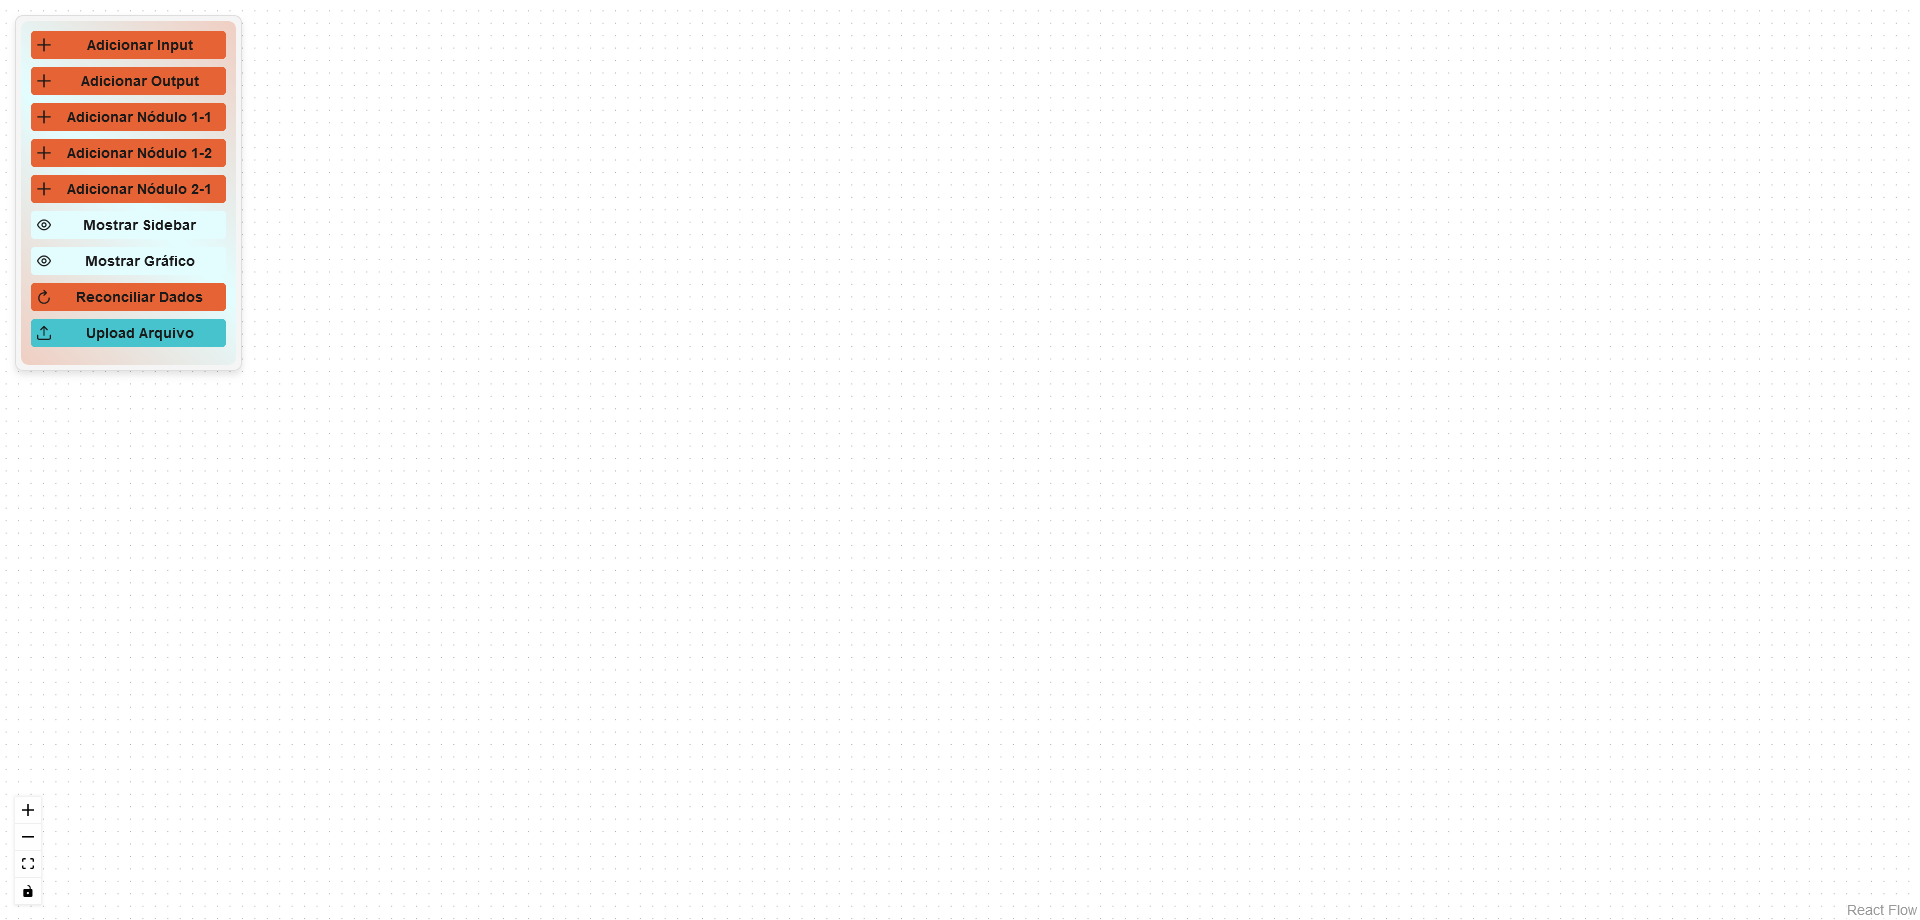
\includegraphics[width=0.8\textwidth]{figuras/empty-canvas.png}
    \caption{Exemplo da área de trabalho no canvas do RADARE (Fonte: próprio autor, 2024).}
    \label{Fig:EmptyCanvas}
\end{figure}

% -------------------------
\subsubsection{Lógica de conexão entre os nódulos no \textit{canvas}}

O sistema permite que o usuário estabeleça conexões visuais entre os nódulos, representando o fluxo de dados entre diferentes pontos de um processo industrial. Essas conexões são fundamentais para assegurar que os dados fluam corretamente entre os elementos do \textit{canvas}, como entradas, saídas e pontos de processamento.

A Figura \ref{Fig:NodeConnections} ilustra a conexão de dois nódulos no \textit{canvas}, demonstrando como o usuário pode arrastar e soltar as conexões de forma intuitiva. O usuário também pode ajustar e mover essas conexões entre os nódulos, proporcionando flexibilidade na organização dos fluxos de dados e permitindo a personalização do layout conforme as necessidades do processo.

O trecho principal do código responsável pela criação dessa funcionalidade está disponível no \textbf{Anexo \ref{Anexo:frontCodeNodeTwoOne}}. Cada conexão entre os nódulos possui um valor e uma tolerância associados, que podem ser modificados diretamente com um duplo clique na linha de conexão, permitindo ao usuário ajustar os parâmetros conforme necessário. Além disso, as conexões recebem nomes gerados automaticamente para facilitar a distinção entre as diferentes \textit{tags}.

\begin{figure}[htbp]
    \centering
    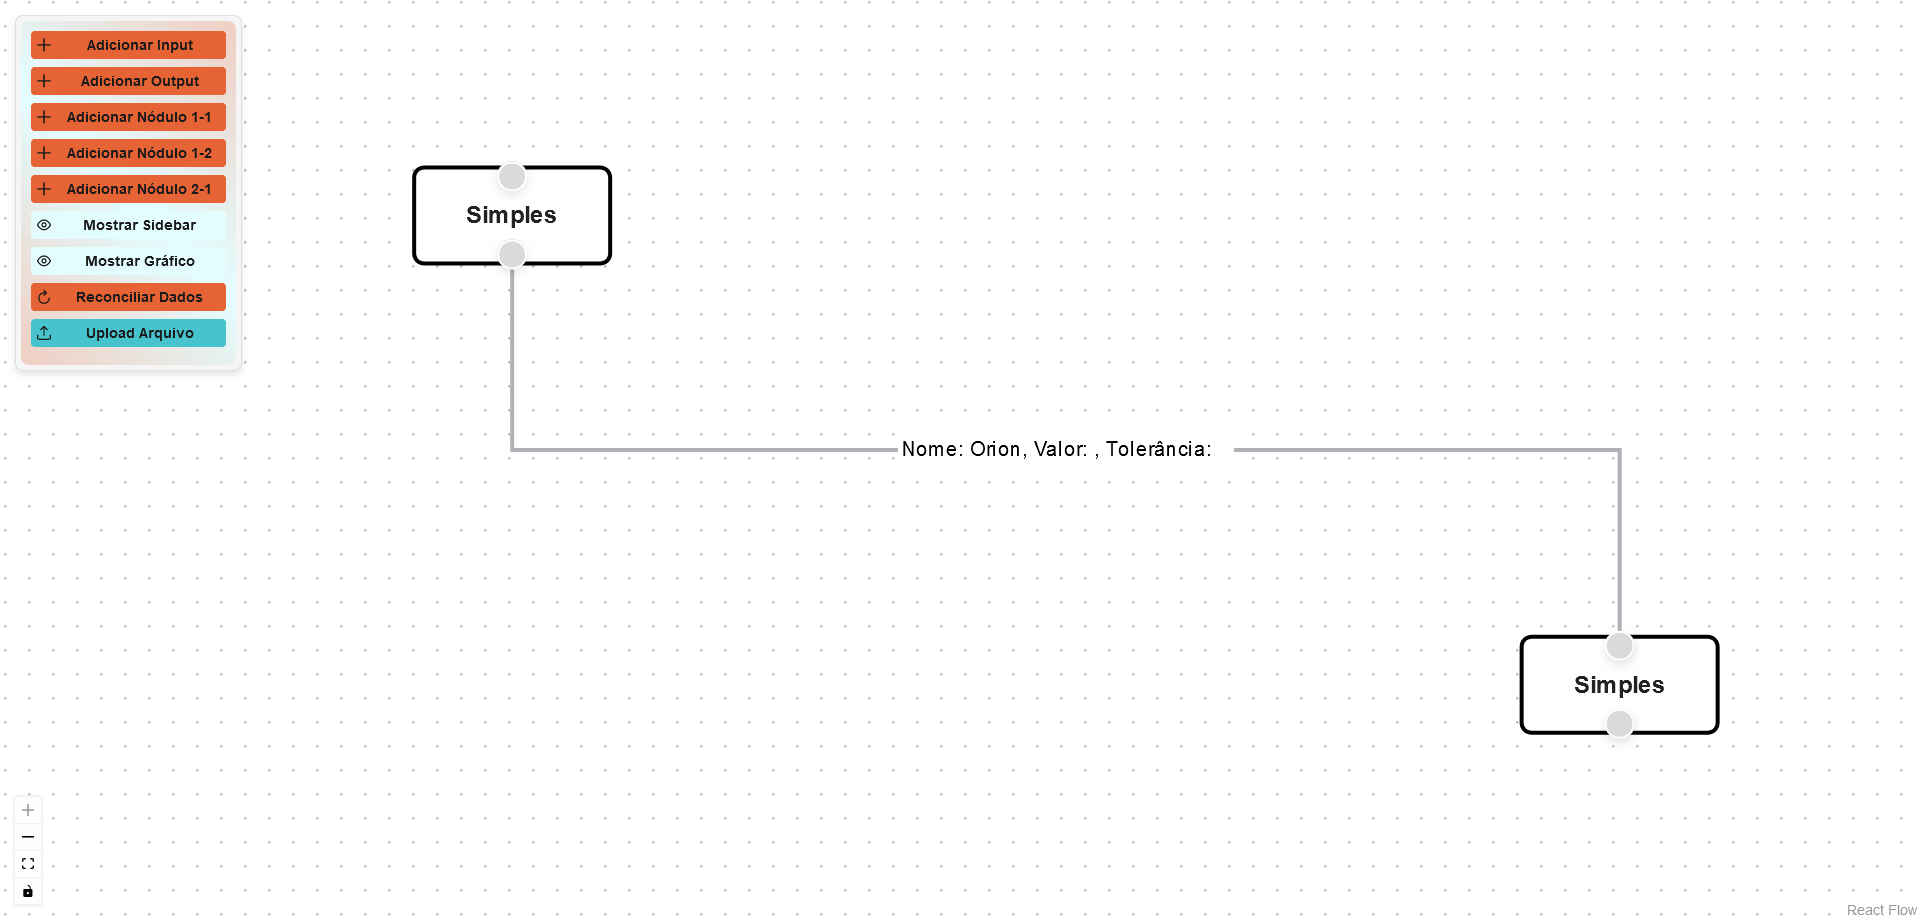
\includegraphics[width=0.8\textwidth]{figuras/node-connection-example.png}
    \caption{Exemplo de conexão entre nódulos no \textit{canvas} (Fonte: próprio autor, 2024).}
    \label{Fig:NodeConnections}
\end{figure}

% -------------------------
\subsection{Interface de Gráfico de Reconciliação de Dados}

A interface de gráfico de reconciliação de dados no RADARE permite ao usuário analisar as interações entre variáveis ao longo do processo de reconciliação. Este gráfico exibe os valores reconciliados e medidos, facilitando a comparação direta entre os dados ajustados e os dados originais. O objetivo é fornecer uma visualização clara e precisa das variações dos dados em função das interações realizadas, permitindo que o usuário identifique rapidamente discrepâncias e avalie a precisão dos dados reconciliados.

A Figura \ref{Fig:ReconciliationGraph} apresenta um exemplo de gráfico de interações versus valores na interface do RADARE. Esse gráfico ilustra como os valores das variáveis mudam em resposta às diferentes interações, oferecendo ao usuário uma ferramenta visual para monitorar e ajustar o processo de reconciliação de dados.

O código principal responsável pela funcionalidade de exibição desse gráfico pode ser encontrado no \textbf{Anexo \ref{Anexo:graphDisplayCode}}.

\begin{figure}[htbp]
    \centering
    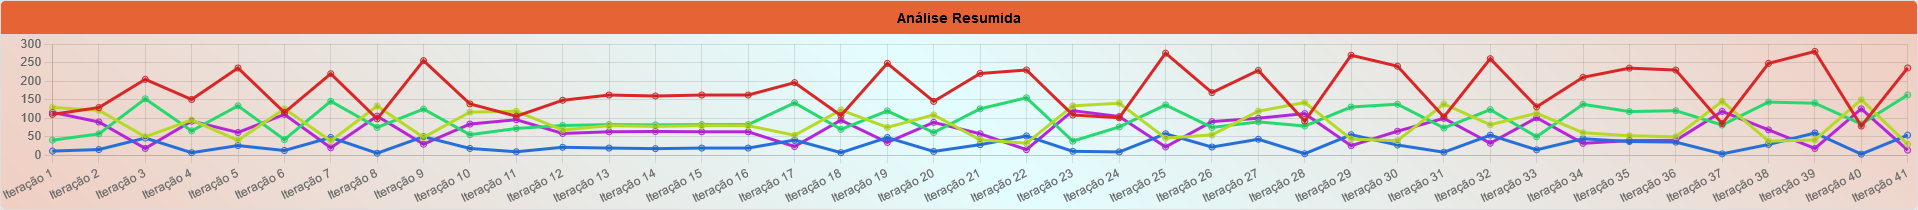
\includegraphics[width=1\textwidth]{figuras/interface-grafico.png}
    \caption{Exemplo do gráfico de reconciliações por interação (Fonte: próprio autor, 2024).}
    \label{Fig:ReconciliationGraph}
\end{figure}

% -------------------------
\subsection{Interface da \textit{sidebar} de informações do sistema}

A \textit{sidebar} de informações do sistema no RADARE serve como um painel auxiliar para exibir informações detalhadas sobre os nódulos e fluxos configurados no \textit{canvas}. Ela permite ao usuário acessar dados adicionais e propriedades de cada elemento, facilitando o monitoramento e o ajuste preciso dos componentes do fluxo de trabalho industrial. A \textit{sidebar} também possibilita uma navegação rápida entre os nódulos e fornece opções para personalização, promovendo uma experiência de uso intuitiva e eficiente.

A Figura \ref{Fig:SidebarInterface} mostra um exemplo da \textit{sidebar} com detalhes de nódulos selecionados, destacando como as informações são organizadas para facilitar a edição e o monitoramento dos elementos visuais do \textit{canvas}. Nos próximos tópicos, aprofundaremos as funcionalidades oferecidas pela \textit{sidebar}, incluindo exemplos de código e explicações sobre a personalização dos nódulos e fluxos. O código que rege a lógica por trás deste componente está disponível no \textbf{Anexo \ref{Anexo:CodigoSidebar}}.

\begin{figure}[htbp]
    \centering
    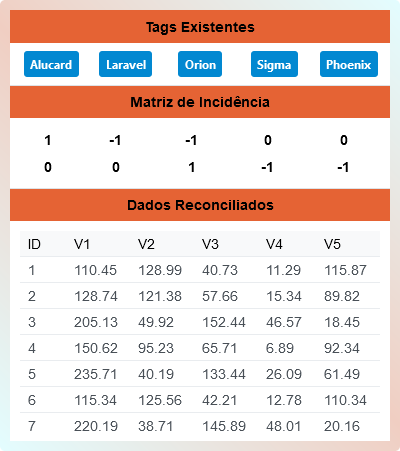
\includegraphics[width=0.4\textwidth]{figuras/interface-sidebar.png}
    \caption{Exemplo da \textit{sidebar} de informações do sistema no RADARE, exibindo dados e opções de configuração de nódulos (Fonte: próprio autor, 2024).}
    \label{Fig:SidebarInterface}
\end{figure}

% -------------------------
\subsection{Resultados finais do front-end em sua visualização completa}

O desenvolvimento do front-end do RADARE culminou em uma tela inicial funcional e intuitiva, integrando todas as funcionalidades discutidas anteriormente para oferecer uma solução prática e eficiente ao usuário. A área do \textit{canvas} serve como o núcleo da interface, permitindo que o usuário visualize, conecte e manipule os nódulos para configurar o fluxo de dados industrial de maneira personalizada. É nesse espaço que os fluxos de trabalho são estruturados, com entradas, saídas e pontos de processamento conectados em harmonia para atender às necessidades específicas dos processos industriais.

A Figura \ref{Fig:CanvasArea} apresenta o \textit{canvas} com vários nódulos interligados, proporcionando uma visão abrangente de como os elementos podem ser organizados e ajustados para criar um fluxo de trabalho viável e eficiente. Cada nódulo desempenha uma função distinta dentro do sistema, e as conexões entre eles representam o fluxo de dados que o RADARE processa e reconcilia. 

Nas seções seguintes, exploraremos as funcionalidades disponíveis no \textit{canvas} de forma detalhada, incluindo a adição de novos nódulos, a interconexão entre eles, a modificação de parâmetros, e a execução de tarefas de reconciliação de dados. Serão apresentados exemplos práticos de código e interações no ambiente, ilustrando como todas essas funcionalidades trabalham em conjunto para oferecer uma solução robusta e eficaz.
 
\begin{figure}[htbp]
    \centering
    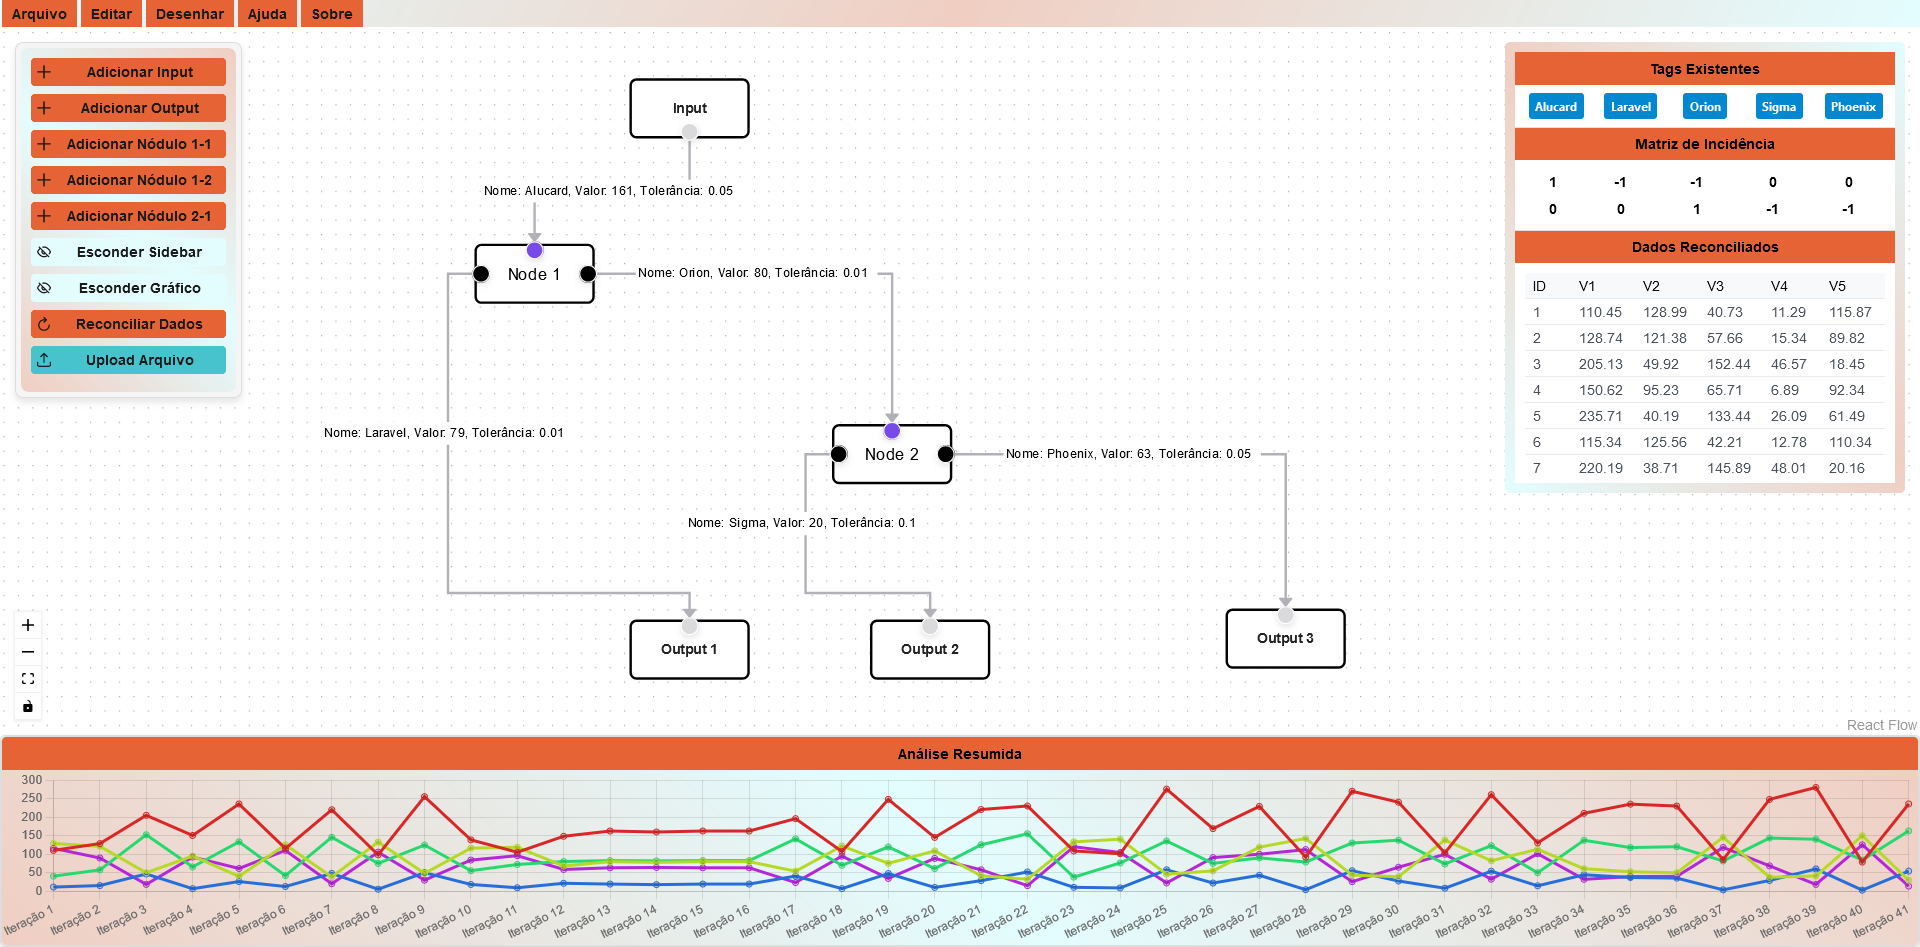
\includegraphics[width=0.8\textwidth]{figuras/interface-completa.png}
    \caption{Exemplo da área de trabalho no canvas do RADARE (Fonte: próprio autor, 2024).}
    \label{Fig:CanvasArea}
\end{figure}

% -------------------------
\section{Resultados do desenvolvimento do \textit{back-end}}

O \textit{back-end} do RADARE foi desenvolvido em \textit{Python} utilizando o \textit{framework} Flask. Essa camada gerencia as requisições da interface, processa os dados submetidos pelo usuário e realiza os cálculos de reconciliação utilizando o método dos multiplicadores de Lagrange. A estrutura foi configurada para responder de maneira eficiente às operações do \textit{front-end}, enviando os resultados dos cálculos e garantindo uma comunicação ágil entre as partes do sistema.

Além de realizar a reconciliação de dados, o \textit{back-end} também gerencia a autenticação e o armazenamento seguro dos dados processados. Com essa estrutura, foi possível assegurar a integridade dos dados e a consistência nos processos realizados, resultando em um sistema robusto e preparado para operações contínuas e de alta demanda.

% -------------------------
\subsection{Desenvolvimento das interfaces RESTful de comunicação entre os sistemas}

As interfaces RESTful foram projetadas para garantir uma comunicação eficiente e segura entre o \textit{front-end} e o \textit{back-end} do sistema RADARE. Cada rota foi cuidadosamente estruturada para facilitar o envio e recebimento de dados, bem como a execução dos processos de reconciliação. Abaixo, são descritas as rotas implementadas, com exemplos de código e explicações detalhadas sobre cada funcionalidade, destacando a importância de cada \textit{endpoint} na integração dos componentes do sistema.

% -------------------------
\subsubsection{Interface RESTful POST /reconcile}

A rota \texttt{POST /reconcile} é responsável por receber os dados dos sensores enviados pelo \textit{front-end} e realizar a reconciliação utilizando o método dos multiplicadores de Lagrange. Após a entrada dos dados, o \textit{back-end} processa as informações e aplica o método para ajustar os valores conforme as restrições impostas, garantindo a consistência dos dados reconciliados. Os resultados obtidos são então armazenados no banco de dados, permitindo a sua recuperação e visualização pelo sistema conforme necessário.

O código completo que implementa essa funcionalidade pode ser consultado no \textbf{Anexo \ref{Anexo:CodigoRouteReconcile}}.

% -------------------------
\subsubsection{Interface RESTful GET /results}

A rota \texttt{GET /results} foi implementada para possibilitar que o usuário recupere os resultados das reconciliações de dados realizadas anteriormente. Ao ser acionada, essa rota consulta o banco de dados e retorna os valores reconciliados, que são então exibidos na interface gráfica, permitindo que o usuário visualize e analise os dados ajustados de forma clara e organizada.

O processo de recuperação desses dados envolve uma consulta ao banco de dados, onde as informações resultantes das reconciliações são armazenadas após o processamento inicial. Esses resultados incluem os valores corrigidos e ajustados por meio do método dos multiplicadores de Lagrange, aplicados durante a fase de reconciliação.

Para mais detalhes sobre o código completo desta rota, consulte o \textbf{Anexo \ref{Anexo:CodigoRouteResults}}, onde é apresentada a implementação completa, incluindo as especificidades da consulta ao banco de dados e a formatação dos dados antes de serem enviados para o \textit{front-end}.

% -------------------------
\subsubsection{Interface RESTful POST /upload}

A rota \texttt{POST /upload} é essencial para o funcionamento do RADARE, pois permite o envio de arquivos CSV contendo dados externos, como leituras de sensores industriais, que serão posteriormente integrados ao banco de dados do sistema. Esses dados servem de base para os processos de reconciliação, possibilitando uma análise precisa e consistente das informações coletadas.

Quando um arquivo é enviado através desta rota, ele é processado no \textit{back-end} para extrair as informações contidas no CSV. Em seguida, os dados são armazenados no banco de dados, ficando disponíveis para as etapas de reconciliação e visualização no \textit{front-end}. Esse fluxo garante que o sistema possa ser atualizado com dados de múltiplas fontes, permitindo uma integração contínua e ampliando a capacidade de análise do RADARE.

O código completo da implementação da rota \texttt{POST /upload} está disponível no \textbf{Anexo \ref{Anexo:CodigoRouteUpload}}.

% -------------------------
\subsection{Serviços desenvolvidos para o sistema}

Os serviços, comumente chamados de \textit{services} no \textit{back-end} são responsáveis por implementar a lógica de negócio, processar os dados e invocar os cálculos de reconciliação. Eles abstraem a complexidade do sistema, garantindo que os dados sejam processados corretamente antes de serem enviados ao banco de dados ou utilizados na interface. Abaixo estão descritos os principais \textit{services} do sistema RADARE, juntamente com exemplos de código e diagramas.

% -------------------------
\subsubsection{Serviço de validação de dados}

O serviço de validação de dados assegura que as informações recebidas estejam no formato apropriado antes de seguirem para o processamento no sistema. Ele verifica a presença de todos os campos obrigatórios, assegura a consistência dos tipos de dados e identifica quaisquer valores ausentes ou inválidos que possam comprometer a integridade do processo de reconciliação. Essa camada de validação é essencial para prevenir erros e garantir que apenas dados confiáveis sejam considerados no cálculo dos resultados.

O trecho principal do código que implementa o serviço de validação de dados pode ser consultado integralmente no \textbf{Anexo \ref{Anexo:CodigoValidacaoDados}}.

% -------------------------
\subsubsection{Serviço de processamento de dados}

O serviço de processamento de dados é responsável por manipular arquivos CSV enviados pelos usuários, convertendo as informações contidas nesses arquivos em estruturas apropriadas para armazenamento no banco de dados e para execução dos cálculos de reconciliação. Este serviço é essencial para garantir que os dados externos sejam integrados ao sistema RADARE de maneira eficaz e que estejam no formato correto para serem processados e analisados.

A validação e transformação dos dados incluem a verificação da consistência dos valores, adequação das colunas conforme os requisitos do banco de dados e conversão dos tipos de dados necessários para as operações de cálculo. Qualquer dado inconsistente ou fora do padrão esperado é tratado antes de ser persistido, assegurando que apenas dados válidos sejam integrados ao sistema.

O trecho principal do código responsável pela criação desse serviço pode ser encontrado em sua totalidade no \textbf{Anexo \ref{Anexo:CodigoProcessamentoDados}}.

% -------------------------
\subsubsection{Serviço de Reconciliação de Dados}

O serviço de reconciliação de dados é uma das funcionalidades centrais do sistema RADARE, sendo responsável por executar o algoritmo de reconciliação utilizando o método dos multiplicadores de Lagrange. Esse método matemático garante que as restrições de balanço de massa e energia sejam rigorosamente respeitadas, assegurando a consistência dos dados processados. Durante a reconciliação, o serviço analisa e ajusta os dados coletados de sensores e outros pontos de entrada, alinhando-os às condições impostas e reduzindo discrepâncias.

Para cada execução, o serviço recebe dados brutos e aplica o algoritmo de reconciliação, retornando valores ajustados que atendem às restrições estabelecidas. Esse processamento permite ao sistema RADARE gerar dados confiáveis e coerentes, essenciais para a análise de processos industriais. 

O código principal deste serviço, detalhado no \textbf{Anexo \ref{Anexo:CodigoReconciliacaoDados}}, exemplifica a implementação do método de reconciliação e a integração com o banco de dados para o armazenamento dos resultados.

% -------------------------
\subsection{Modelos desenvolvidos para o sistema}

Os \textit{models} foram implementados utilizando uma ORM (Object-Relational Mapping) em \textit{Python} para facilitar a comunicação com o banco de dados PostgreSQL. Esse método permite mapear objetos do código para tabelas no banco de dados, tornando o desenvolvimento mais ágil e a manutenção mais eficiente. Os principais modelos implementados no sistema incluem:

\begin{itemize}
    \item \textbf{Process Model}: Representa os processos industriais, contendo as informações de variáveis medidas e parâmetros relevantes.
    \item \textbf{Measurement Model}: Armazena as medições recebidas dos sensores, assegurando que cada registro seja associado ao respectivo processo.
    \item \textbf{Result Model}: Registra os resultados das reconciliações, vinculando-os aos processos e medições correspondentes para consulta futura.
\end{itemize}

O trecho principal do código responsável pela criação desses modelos pode ser encontrado em sua totalidade no \textbf{Anexo \ref{Anexo:CodigoModelo}}.

% -------------------------
\section{Resultados do desenvolvimento do banco de dados}

O banco de dados utilizado no sistema RADARE foi implementado em PostgreSQL e armazena todas as informações relevantes para a execução do processo de reconciliação de dados industriais, gerenciamento de usuários e rastreamento de atividades. A modelagem foi feita de forma a garantir a integridade e eficiência na consulta e manipulação dos dados. A seguir, são descritas as principais tabelas implementadas no sistema.

% -------------------------
\subsection{Tabela de Dados de Processos}

A tabela de dados de processos industriais (\autoref{tab:processDataTable}) armazena informações essenciais para o funcionamento do sistema RADARE, incluindo medições de sensores e os resultados das reconciliações de dados. Esta estrutura permite uma organização clara e precisa dos dados, garantindo que cada registro seja identificado de forma única e possa ser associado a operações de reconciliação específicas.

\begin{table}[htbp]
    \centering
    \caption{Descrição das colunas da tabela de dados de processos industriais.}
    \label{tab:processDataTable}
    \begin{tabular}{|l|p{10cm}|}
        \hline
        \textbf{Coluna} & \textbf{Descrição} \\ \hline
        \textbf{id} & Identificação única do registro, usada como chave primária. \\ \hline
        \textbf{user} & Identifica o usuário responsável pela reconciliação. \\ \hline
        \textbf{time} & Horário da reconciliação, para referência temporal. \\ \hline
        \textbf{tagname} & Nome da variável medida (sensor ou ponto de coleta). \\ \hline
        \textbf{tagreconciled} & Valor reconciliado da variável após ajustes. \\ \hline
        \textbf{tagcorrection} & Valor da correção aplicada à variável medida. \\ \hline
        \textbf{tagmatrix} & Matriz de correlação usada na reconciliação. \\ \hline
    \end{tabular}
\end{table}


% -------------------------
\subsection{Tabela de Usuários}

A tabela de usuários (\autoref{Tab:Users}) é essencial para gerenciar a autenticação, as permissões e o rastreamento de atividades dos usuários no sistema RADARE. Essa estrutura não apenas assegura que apenas usuários autorizados possam acessar determinadas funcionalidades, mas também facilita a auditoria e a segurança do sistema, mantendo informações sensíveis e essenciais para o controle de acesso.

\begin{table}[htbp]
    \centering
    \caption{Estrutura da tabela de usuários no sistema RADARE.}
    \label{Tab:Users}
    \begin{tabular}{|l|p{10cm}|}
        \hline
        \textbf{Coluna} & \textbf{Descrição} \\ \hline
        \textbf{id} & UUID único para cada usuário (chave primária). \\ \hline
        \textbf{username} & Nome de usuário para login (deve ser único). \\ \hline
        \textbf{email} & Endereço de email para notificações. \\ \hline
        \textbf{password\_hash} & Hash da senha para segurança. \\ \hline
        \textbf{role} & Função do usuário (e.g., admin, operador, analista). \\ \hline
        \textbf{created\_at} & Data e hora da criação da conta. \\ \hline
        \textbf{last\_login} & Data e hora do último acesso. \\ \hline
    \end{tabular}
\end{table}

% -------------------------
\subsection{Tabela de Logs de Atividade}

A tabela de logs de atividade (Tabela \ref{Tab:ActivityLogs}) armazena registros detalhados das ações realizadas pelos usuários no sistema, permitindo auditoria e rastreamento de atividades como uploads de arquivos ou execuções de reconciliação de dados. Essa estrutura auxilia no monitoramento e na segurança, facilitando a análise das interações dos usuários com o sistema.

\begin{table}[htbp]
    \centering
    \caption{Estrutura da tabela de logs de atividade no sistema RADARE.}
    \label{Tab:ActivityLogs}
    \begin{tabular}{|l|p{10cm}|}
        \hline
        \textbf{Coluna} & \textbf{Descrição} \\ \hline
        \textbf{id} & Identificação única para cada log de atividade. \\ \hline
        \textbf{user\_id} & Referência ao ID do usuário que realizou a ação. \\ \hline
        \textbf{action} & Descrição da ação realizada. \\ \hline
        \textbf{timestamp} & Data e hora da realização da ação. \\ \hline
        \textbf{details} & Informações adicionais sobre a ação. \\ \hline
    \end{tabular}
\end{table}

% -------------------------
\subsection{Tabela de Configurações de Processos}

A tabela de configurações de processos industriais (Tabela \ref{Tab:ProcessConfigurations}) armazena parâmetros essenciais para a personalização do sistema, incluindo limites de variáveis e especificações de medições. Essa estrutura permite adaptar o comportamento do sistema a diferentes cenários industriais, proporcionando flexibilidade na definição de cada processo.

\begin{table}[htbp]
    \centering
    \caption{Estrutura da tabela de configurações de processos no sistema RADARE.}
    \label{Tab:ProcessConfigurations}
    \begin{tabular}{|l|p{10cm}|}
        \hline
        \textbf{Coluna} & \textbf{Descrição} \\ \hline
        \textbf{id} & Identificação única para cada configuração de processo. \\ \hline
        \textbf{process\_name} & Nome do processo industrial específico. \\ \hline
        \textbf{sensor\_limits} & Limites definidos para as variáveis dos sensores. \\ \hline
        \textbf{created\_by} & ID do usuário responsável pela criação da configuração. \\ \hline
        \textbf{created\_at} & Data e hora em que a configuração foi registrada no sistema. \\ \hline
    \end{tabular}
\end{table}

% -------------------------
\section{Manuais de sistema}

Como parte do desenvolvimento do \textit{software} RADARE, foram criados dois manuais distintos para auxiliar tanto os administradores técnicos quanto os usuários finais na utilização e manutenção do sistema. Esses manuais visam garantir a correta operação e longevidade da aplicação, fornecendo instruções claras sobre o funcionamento do sistema e as melhores práticas para sua utilização.

% -------------------------
\subsection{Manual de manutenção do sistema}

O manual de manutenção do sistema fornece orientações para desenvolvedores e administradores sobre as funções internas do RADARE, incluindo detalhes sobre o *front-end*, *back-end* e banco de dados. Ele descreve as principais funções, fluxos de dados e interações entre os componentes, além de instruções para manutenção, como atualização de bibliotecas, ajustes de configurações, monitoramento de logs e execução de testes de desempenho. Também aborda limitações técnicas, como número máximo de conexões simultâneas e requisitos mínimos de hardware. Procedimentos para diagnóstico e resolução de problemas comuns, como erros de reconciliação e falhas no processamento de arquivos, são apresentados.

O manual completo está disponível no \textbf{Anexo \ref{Cap:manualManutencao}}, facilitando a consulta detalhada sobre a manutenção do sistema.

% -------------------------
\subsection{Manual de uso para o usuário final}

O manual de uso foi elaborado para orientar o usuário nas tarefas de reconciliação de dados industriais com o *RADARE*. Ele apresenta uma introdução ao sistema, explicando seu propósito e principais funcionalidades. Em seguida, descreve o passo a passo das operações, incluindo instruções para adicionar nódulos no \textit{canvas}, realizar reconciliações e carregar arquivos CSV.

O manual inclui guias visuais e dicas de usabilidade, auxiliando na navegação e no uso eficiente da interface, além de oferecer soluções para problemas comuns, como erros de upload e falhas de conexão entre nódulos. 

O manual completo está disponível para consulta no \textbf{Anexo \ref{Anexo:manualUsuario}}, com todos os detalhes necessários para o uso do sistema.
